\documentclass{standalone}
\usepackage{mintikz}

\tikzset{every picture/.style={thick}}

\def\A{0.25}
\def\Q{10}
\def\wo{1e3}
\def\fo{\wo/2*pi}

\begin{document}
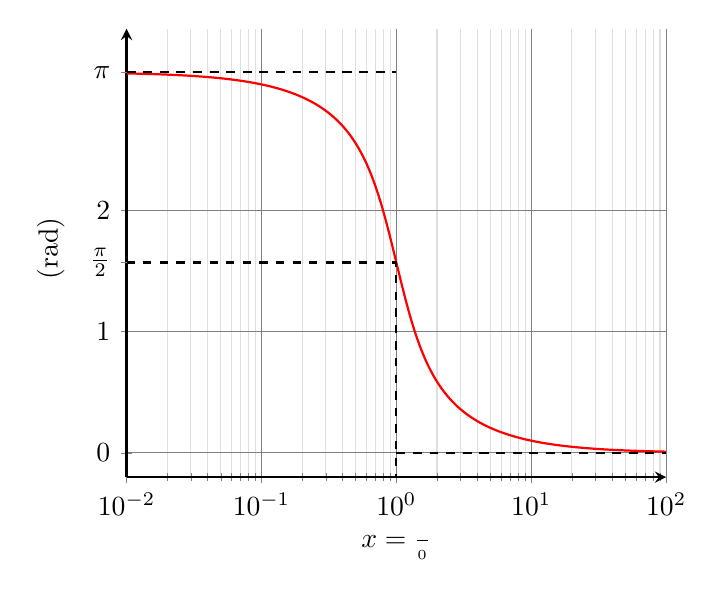
\begin{tikzpicture}[]
	\begin{semilogxaxis}[
			xmin=1e-2, xmax=1e2,
			% xticklabels={\num{e-1}, \num{e3}, \num{e4}},
			% extra x ticks={5e2, 5e3},
			% extra x tick labels={\num{5e2}, \num{5e3}},
			% extra x tick style={grid=minor, grid style={gray!25}, font=\tiny},
			ymin=-0.2, ymax=3.5,
			ytick={0, 1, 2},
			extra y ticks={1.57079, 3.1415},
			extra y tick labels={$\DS\frac{\pi}{2}$, $\pi$},
			extra y tick style={grid=none},
			xlabel={$x = \DS\frac{\w}{\w_0}$}, ylabel=$\f$ (rad),
			axis lines=left,
			grid=both,
			minor grid style={gray!25},
			major grid style={black!50},
			% width=10cm,
			% height=7cm,
			clip=true]
		\addplot[
			domain=1e-2:1e2,
			smooth, samples=500, red, thick]
		{pi/2-atan(\x-1/\x)*pi/180};
		\addplot[
			domain=1e-2:1e0,
			smooth, samples=500, dashed, thick]
		{pi};
		\addplot[
			domain=1e0:1e2,
			smooth, samples=500, dashed, thick]
		{0};
		\draw[thick, dashed]
		(axis cs:1e-2,1.57079) -|
		(axis cs:1,-0.2);
	\end{semilogxaxis}
\end{tikzpicture}
\end{document}
